\documentclass[12pt]{amsart}

\usepackage[
	paperheight=11in,
	paperwidth=8.5in,
	inner=0.4in,
	textheight=10.2in,
	textwidth=7.5in,
	% marginparwidth=120pt,
	% marginparsep=32pt,
	% bottom=1.4in,
	% left=0.5in,
	% right=0.5in,
	% footskip=1.0in
]{geometry}
\geometry{letterpaper}

\usepackage{array}
\usepackage{amssymb}
\usepackage{asymptote}
\usepackage{amsmath}
\usepackage{amsfonts}
\usepackage{animate}
\usepackage{arrayjobx}
\usepackage{arydshln}
\usepackage{bookman}
\usepackage{color}
\usepackage{cancel}
\usepackage{calculator}
\usepackage{collcell}
\usepackage{epstopdf}
\usepackage{enumerate}
\usepackage{epsfig}
\usepackage[english]{babel}
\usepackage{etoolbox}
\usepackage{fancyhdr}
\usepackage{fancybox}
\usepackage[nomessages]{fp}
\usepackage{graphics}
\usepackage{graphicx}
\usepackage{ifthen}
\usepackage{ifmtarg}
\usepackage[latin1]{inputenc}
\usepackage{latexsym}
\usepackage{multirow}
\usepackage{multicol}
\usepackage{multimedia}
\usepackage{mathbbol}
\usepackage{mathtools}
\usepackage{multido}
\usepackage{palatino}
\usepackage{polynom}
\usepackage{pxfonts}
\usepackage{pifont}
\usepackage{pgffor}
\usepackage{pdfpages}
\usepackage[parfill]{parskip}
\usepackage{soul}
\usepackage{tikz}
\usetikzlibrary{arrows,shapes,trees,shapes.geometric,calc}
\usepackage{txfonts}
\usepackage{tcolorbox}
\usepackage{wasysym}
\usepackage{wrapfig}
\usepackage{xcolor}
\usepackage{xmpmulti}
\usepackage{xparse}
\usepackage{xstring}
\usepackage{mathrsfs}
\newcommand{\LAP}[1]{\mathscr{L}\{#1\}}

\renewcommand{\headrulewidth}{0pt} % remove lines as well

\numberwithin{equation}{section}

\DeclareGraphicsRule{.tif}{png}{.png}{`convert #1 `dirname #1`/`basename #1 .tif`.png}

\def\plottingAxes{
	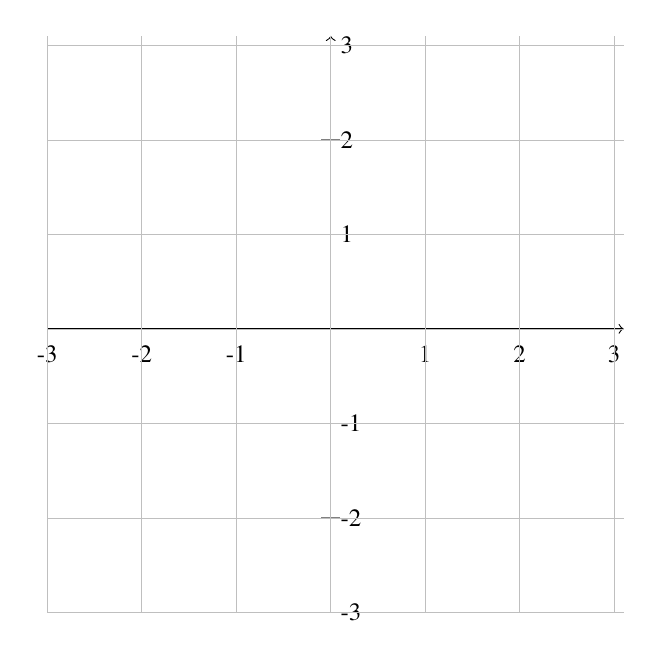
\begin{tikzpicture}[samples=100, scale=1.2]

		% === figure/domain/tick bounds ===
		\def\tmin{-3.0}	\def\tmax{3.1}
		\def\ymin{-3.0}	\def\ymax{3.1}
		\def\tticks{-3, -2, -1, 1, 2, 3}
		\def\yticks{-3, -2, -1, 1, 2, 3}

		% === Axes ===
		\draw[->] (\tmin	,0		) -- (\tmax	,0		);
		\draw[->] (0		,\ymin	) -- (0		,\ymax	);
		% \node[font=\small, below] at (\tmax - 0.1	, 0) {$t$};

		% === Tick marks/numeric labels ===
		\foreach \t in \tticks {
			\draw[gray]	(\t,0.1) -- (\t,-0.1);					% t ticks
			\node[below, font=\small] at (\t,-0.08) {\t};	% t labels
			
		}
		\foreach \y in \yticks {
			\draw[gray]	(0.1,\y) -- (-0.1,\y);				% y ticks
			\node[right, font=\small] at (0,\y) {\y};	% y labels
		}
		\draw[very thin,color=lightgray] (\tmin,\ymin) grid (\tmax,\ymax);	
	\end{tikzpicture}
}

\def\slopefieldA{
		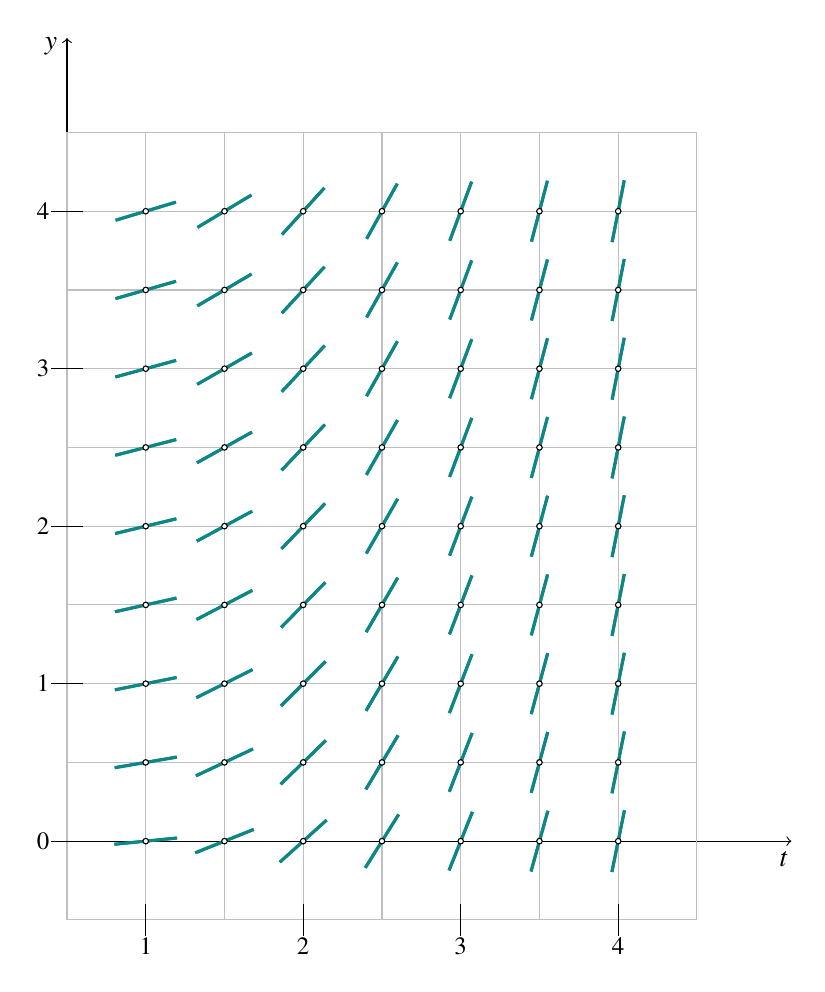
\begin{tikzpicture}[declare function={f(\x,\y) = 0.1*sqrt(\y) + 0.4*\x*\x;}, scale=2]

			\pgfkeys{/pgf/number format/.cd,
				fixed,
				precision=0
			}
			\def\tmin{0} \def\tmax{4}
			\def\ymin{-0.5} \def\ymax{4.5}
			\def\tmargin{0.5} % extra space around the grid
			\def\ymargin{0.5} % extra space around the grid
			\def\nt{6}  \def\ny{8}
			\def\arrowscale{0.4} % length of slope arrows

			% stepsize along t-axis and y-axis
			\pgfmathsetmacro{\tL}{\tmin + \tmargin}
			\pgfmathsetmacro{\tR}{\tmax - \tmargin}
			\pgfmathsetmacro{\yL}{\ymin + \ymargin}
			\pgfmathsetmacro{\yR}{\ymax - \ymargin}
			\pgfmathsetmacro{\tstep}{(\tR-\tL)/\nt}
			\pgfmathsetmacro{\ystep}{(\yR-\yL)/\ny}

			% Draw grid lines
			\foreach \i in {0.5,1.0,...,3.5} {
				\draw[thin, gray!50] (\i, \ymin) -- (\i, \ymax);
			}
			\foreach \j in {0,...,\ny} {
				\pgfmathsetmacro{\yk}{\yL + \j * \ystep}
				\draw[thin, gray!50] (\tmin, \yk) -- (\tmax, \yk);
			}

			% Axes
			\draw[->] (\tmin, 0) -- (\tmax+0.6, 0) node[xshift=-0.1cm, below] {$t$};
			\draw[->] (0, \ymin) -- (0, \ymax+0.6) node[yshift=-0.1cm, left] {$y$};

			% Bounding box
			\draw[gray!50] (\tmin,\ymin) rectangle (\tmax,\ymax);

			% Tick marks and labels on t-axis
			\foreach \t in {\tL,...,\tR} {
				\pgfmathparse{\t < 0}
				\ifnum\pgfmathresult=1	 % shift negative ticks
					\draw (\t,\ymin-0.1) -- (\t,\ymin+0.1)
					node[font=\small, below, xshift=-0.15cm, yshift=-0.1cm] {\pgfmathprintnumber{\t}};
				\else
					\draw (\t,\ymin-0.1) -- (\t,\ymin+0.1)
					node[font=\small, below, yshift=-0.3cm] {\pgfmathprintnumber{\t}};
				\fi
			}

			% Tick marks and labels on y-axis
			\foreach \y in {\yL,...,\yR}
				\draw (\tmin-0.1,\y) -- (\tmin+0.1,\y)
				node[font=\small, left, xshift=-0.3cm] {\pgfmathprintnumber{\y}};

			% Title
			% \node[above, font=\small\bfseries] at (current bounding box.north) 
			% 	{Slope field for \quad $\dfrac{dy}{dx} = 0.1\sqrt{y} + 0.4x^2$};

			% slope field: just draw a vector at each point
			\foreach \i in {0,...,\nt}
			\foreach \j in {0,...,\ny}{
				%
				\pgfmathsetmacro{\tpt}{\tL + \i * \tstep}
				\pgfmathsetmacro{\ypt}{\yL + \j * \ystep}
				% 
				\pgfmathsetmacro{\slope}{f(\tpt,\ypt)}
				% 
				% Normalize direction vector (1, slope) to fixed length
				\pgfmathsetmacro{\len}{sqrt(1 + (\slope)^2)}
				\pgfmathsetmacro{\dt}{\arrowscale / \len}
				\pgfmathsetmacro{\dy}{\arrowscale * \slope / \len}
				% 
				\draw[teal!90, -, line width=1.1pt, shift={(\tpt,\ypt)}] (-0.5*\dt, -0.5*\dy) -- (0.5*\dt, 0.5*\dy);
				\draw[teal!95, line width=1.1pt, shift={(\tpt,\ypt)}] (-0.5*\dt, -0.5*\dy) -- (0.5*\dt, 0.5*\dy);
				\draw[fill=white!50] (\tpt,\ypt) circle (0.5pt);
				% 
			}
		\end{tikzpicture}
}

\def\slopefieldB{
	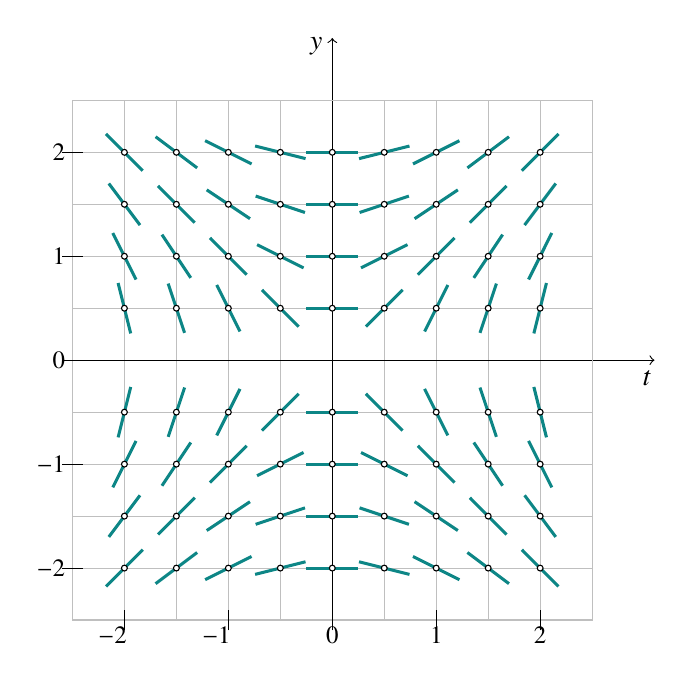
\begin{tikzpicture}[declare function={f(\x,\y)=\x/\y;}, scale=1.32]

		\pgfkeys{/pgf/number format/.cd,
			fixed,
			precision=0
		}
		\def\tmin{-2.5} \def\tmax{2.5}
		\def\ymin{-2.5} \def\ymax{2.5}
		\def\tmargin{0.5} % extra space around the grid
		\def\ymargin{0.5} % extra space around the grid
		\def\nt{8}  \def\ny{8}
		\def\arrowscale{0.5} % length of slope arrows

		% stepsize along t-axis and y-axis
		\pgfmathsetmacro{\tL}{\tmin + \tmargin}
		\pgfmathsetmacro{\tR}{\tmax - \tmargin}
		\pgfmathsetmacro{\yL}{\ymin + \ymargin}
		\pgfmathsetmacro{\yR}{\ymax - \ymargin}
		\pgfmathsetmacro{\tstep}{(\tR-\tL)/\nt}
		\pgfmathsetmacro{\ystep}{(\yR-\yL)/\ny}

		% Draw grid lines
		\foreach \i in {0,...,\nt} {
			\pgfmathsetmacro{\tk}{\tL + \i * \tstep}
			\draw[thin, gray!50] (\tk, \ymin) -- (\tk, \ymax);
		}
		\foreach \j in {0,...,\ny} {
			\pgfmathsetmacro{\yk}{\yL + \j * \ystep}
			\draw[thin, gray!50] (\tmin, \yk) -- (\tmax, \yk);
		}

		% Axes
		\draw[->] (\tmin, 0) -- (\tmax+0.6, 0) node[xshift=-0.1cm, below] {$t$};
		\draw[->] (0, \ymin) -- (0, \ymax+0.6) node[yshift=-0.1cm, left] {$y$};

		% Bounding box
		\draw[gray!50] (\tmin,\ymin) rectangle (\tmax,\ymax);

		% Tick marks and labels on t-axis
		\foreach \t in {\tL,...,\tR} {
			\pgfmathparse{\t < 0}
			\ifnum\pgfmathresult=1	 % shift negative ticks
				\draw (\t,\ymin-0.1) -- (\t,\ymin+0.1)
				node[font=\small, below, xshift=-0.15cm, yshift=-0.1cm] {\pgfmathprintnumber{\t}};
			\else
				\draw (\t,\ymin-0.1) -- (\t,\ymin+0.1)
				node[font=\small, below, yshift=-0.1cm] {\pgfmathprintnumber{\t}};
			\fi
		}

		% Tick marks and labels on y-axis
		\foreach \y in {\yL,...,\yR}
			\draw (\tmin-0.1,\y) -- (\tmin+0.1,\y)
			node[font=\small, left, xshift=-0.1cm] {\pgfmathprintnumber{\y}};

		% Title
		%\node[above, font=\small\bfseries] at (current bounding box.north) 
		%	{Slope field for \quad $y' = x + y$};

		% slope field: just draw a vector at each point
		\foreach \i in {0,...,\nt}
		\foreach \j in {0,...,\ny}{

			\pgfmathsetmacro{\tpt}{\tL + \i * \tstep}
			\pgfmathsetmacro{\ypt}{\yL + \j * \ystep}
			
			\pgfmathparse{\ypt != 0} % avoid division by zero
			\ifnum\pgfmathresult=1
				\pgfmathsetmacro{\slope}{f(\tpt,\ypt)}

				% Normalize direction vector (1, slope) to fixed length
				\pgfmathsetmacro{\len}{sqrt(1 + (\slope)^2)}
				\pgfmathsetmacro{\dt}{\arrowscale / \len}
				\pgfmathsetmacro{\dy}{\arrowscale * \slope / \len}

				%\draw[teal!90, -stealth, line width=1.1pt, shift={(\tpt,\ypt)}] (-0.5*\dt, -0.5*\dy) -- (0.5*\dt, 0.5*\dy);
				\draw[teal!95, line width=1.1pt, shift={(\tpt,\ypt)}] (-0.5*\dt, -0.5*\dy) -- (0.5*\dt, 0.5*\dy);
				\draw[fill=white!50] (\tpt,\ypt) circle (0.8pt);
			\else
				% do nothing (skip this point)
			\fi

		}

	\end{tikzpicture}
}

\def\slopefieldC{
	\resizebox{15cm}{9cm}{%
		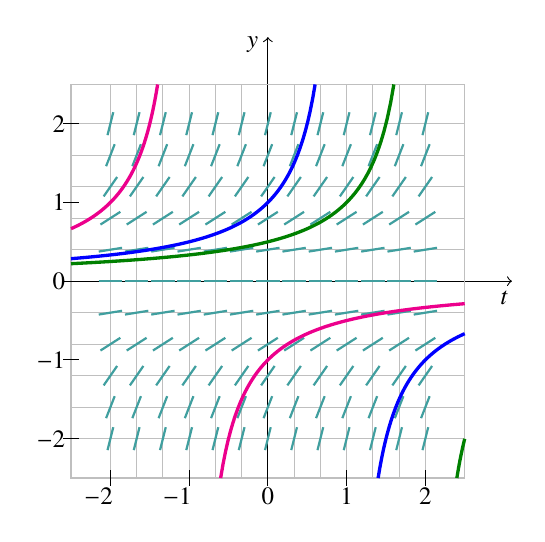
\begin{tikzpicture}[declare function={f(\x,\y)=\y*\y;}, scale=1]

			\pgfkeys{/pgf/number format/.cd,
				fixed,
				precision=1
			}
			\def\tmin{-2.5} \def\tmax{2.5}
			\def\ymin{-2.5} \def\ymax{2.5}
			\def\tmargin{0.5} \def\ymargin{0.5} % extra space around the grid
			\def\nt{12}  \def\ny{10}
			\def\arrowscale{0.3} % length of slope arrows

			% stepsize along t-axis and y-axis
			\pgfmathsetmacro{\tL}{\tmin + \tmargin}
			\pgfmathsetmacro{\tR}{\tmax - \tmargin}
			\pgfmathsetmacro{\yL}{\ymin + \ymargin}
			\pgfmathsetmacro{\yR}{\ymax - \ymargin}
			\pgfmathsetmacro{\tstep}{(\tR-\tL)/\nt}
			\pgfmathsetmacro{\ystep}{(\yR-\yL)/\ny}

			% Draw grid lines
			\foreach \i in {0,...,\nt} {
				\pgfmathsetmacro{\tk}{\tL + \i * \tstep}
				\draw[thin, gray!50] (\tk, \ymin) -- (\tk, \ymax);
			}
			\foreach \j in {0,...,\ny} {
				\pgfmathsetmacro{\yk}{\yL + \j * \ystep}
				\draw[thin, gray!50] (\tmin, \yk) -- (\tmax, \yk);
			}

			% Axes
			\draw[->] (\tmin, 0) -- (\tmax+0.6, 0) node[xshift=-0.1cm, font=\small, below] {$t$};
			\draw[->] (0, \ymin) -- (0, \ymax+0.6) node[yshift=-0.1cm, font=\small, left] {$y$};

			% Bounding box
			\draw[gray!50] (\tmin,\ymin) rectangle (\tmax,\ymax);

			% Tick marks and labels on t-axis
			\pgfmathtruncatemacro{\tLint}{\tL}
			\pgfmathtruncatemacro{\tRint}{\tR}
			\foreach \t in {\tLint,...,\tRint} {
			\pgfmathparse{\t < 0}
			\ifnum\pgfmathresult=1	 % shift negative ticks
				\draw (\t,\ymin-0.1) -- (\t,\ymin+0.1)
				node[font=\small, below, xshift=-0.15cm, yshift=-0.1cm] {\pgfmathprintnumber{\t}};
			\else
				\draw (\t,\ymin-0.1) -- (\t,\ymin+0.1)
				node[font=\small, below, yshift=-0.1cm] {\pgfmathprintnumber{\t}};
			\fi
			}

			% Tick marks and labels on y-axis
			\pgfmathtruncatemacro{\yLint}{\yL}
			\pgfmathtruncatemacro{\yRint}{\yR}
			\foreach \y in {\yLint,...,\yRint}
				\draw (\tmin-0.1,\y) -- (\tmin+0.1,\y)
				node[font=\small, left, xshift=-0.05cm] {\pgfmathprintnumber{\y}};

			% slope field: just draw a vector at each point
			\foreach \i in {0,...,\nt}
			\foreach \j in {0,...,\ny}{

				\pgfmathsetmacro{\tpt}{\tL + \i * \tstep}
				\pgfmathsetmacro{\ypt}{\yL + \j * \ystep}
				\pgfmathsetmacro{\slope}{f(\tpt,\ypt)}

				% Normalize direction vector (1, slope) to fixed length
				\pgfmathsetmacro{\len}{sqrt(1 + (\slope)^2)}
				\pgfmathsetmacro{\dt}{\arrowscale / \len}
				\pgfmathsetmacro{\dy}{\arrowscale * \slope / \len}

				%\draw[teal!60, arrows = {-Stealth[width=4pt, length=4pt, inset=3pt]}, line width=0.8pt, shift={(\tpt,\ypt)}] (-0.5*\dt, -0.5*\dy) -- (0.5*\dt, 0.5*\dy);
				\draw[teal!75, line width=0.8pt, shift={(\tpt,\ypt)}] (-0.5*\dt, -0.5*\dy) -- (0.5*\dt, 0.5*\dy);
				%\draw[fill=white!50] (\tpt,\ypt) circle (1.5pt);
			}

			% Optional solution curves
			\def\yoA{-1}
			\draw[magenta, very thick, samples=100]
				plot[domain=-0.6:\tmax] (\x, {1/(-\x + 1/\yoA)});
			\draw[magenta, very thick, samples=100]
				plot[domain=\tmin:-1.4] (\x, {1/(-\x + 1/\yoA)});

			\def\yoB{0.5}
			\draw[green!50!black, very thick, samples=100]
				plot[domain=\tmin:1.6] (\x, {1/(-\x + 1/\yoB)});
			\draw[green!50!black, very thick, samples=100]
				plot[domain=2.4:\tmax] (\x, {1/(-\x + 1/\yoB)});

			\def\yoC{1}
			\draw[blue, very thick, samples=100]
				plot[domain=\tmin:0.6] (\x, {1/(-\x + 1/\yoC)});
			\draw[blue, very thick, samples=100]
				plot[domain=1.4:\tmax] (\x, {1/(-\x + 1/\yoC)});

		\end{tikzpicture}
	}%
}

\begin{document}

	\pagestyle{empty}

	\hrule
	\begin{center}
		\begin{tabular}{p{6.8in}}
			\multicolumn{1}{c}{\sc Differential Equations} \\
			\multicolumn{1}{c}{\sc Euler's Method}
		\end{tabular}
	\end{center}
	\medskip
	\hrule

	\medskip

	\noindent  Consider the initial value problem with correesponding slope field:
	\[ \frac{dy}{dx} = 0.1\sqrt{y} + 0.4x^2, \hspace{1cm} y(1) = 0.5. \]
		\begin{center}
			% 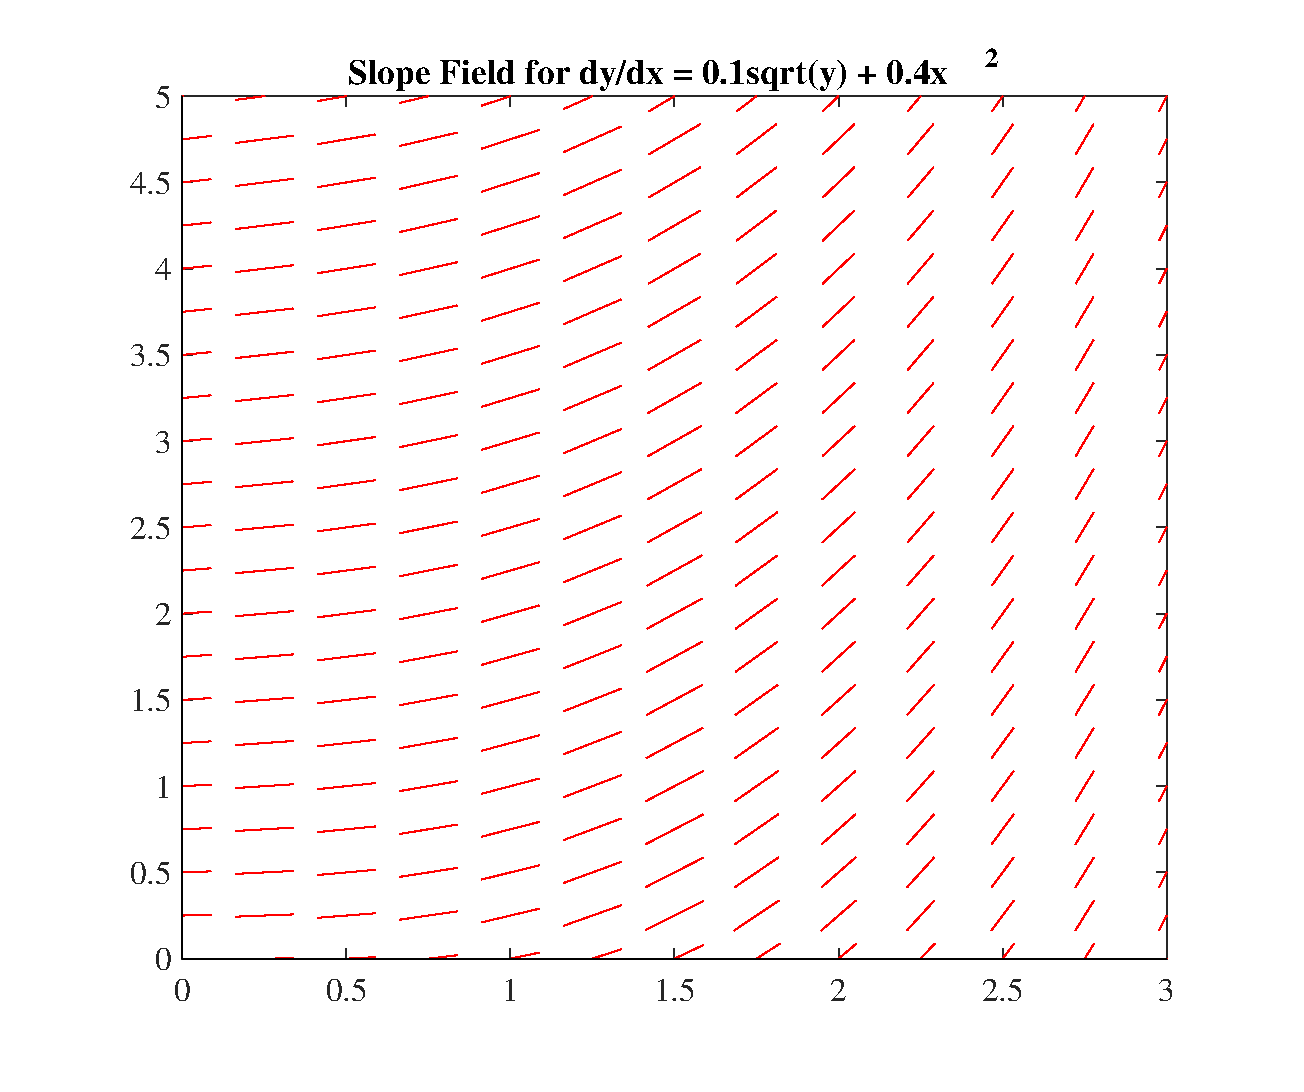
\includegraphics[scale = 0.6, trim = 0in 0in 0in 0in]{figs/DE_E.eps}\\
			\slopefieldA
		\end{center}
		
	\begin{enumerate}
		
		\item On the slope field above, mark the point $P_0$ indicating the initial condition of the solution.

		\item What is the slope $m_0$ of the solution curve at the point $P_0$? \label{Q3}
		\vspace{1in}

		\item Give the equation of a line with slope $m$ that passes through the point $P_0 = (x_0,y_0)$: 
		\vspace{1in}

		\newpage

		\item  Find the equation of this tangent line $L_0$.  Keep in mind that we know the line passes through
		the point $P_0 = (1, 0.5)$ and has the slope $m_0$ that you found in question \ref{Q3}.
		\vspace{1in}

		\item Since the tangent line at $P_0 = (1, 0.5)$ shows the direction the solution moves at $P_0,$ then we
		can approximate another nearby point $P_1$ on the solution curve. Find the point $P_1$ on $L_0$ that has $x$-coordinate only half a unit away, i.e., when $x = 1.5.$
		\vspace{1in}
			
		{\it There is no guarantee that the solution passes through $P_1$, it is just an \textbf{approximation}.}
			
		\item On the slope field, mark the point $P_1$ and sketch the part of the line $L_0$ that lies between 
		$P_0$ and $P_1.$
	\end{enumerate}

	\noindent So, we started at	$P_0,$ and we found the slope and tangent line there. Moving in this direction over a small $x$ distance, gave us another point $P_1$. We can repeat this process at $P_1$ to	approximate another point $P_2,$ as follows:

		\begin{enumerate}
			\item  Find the slope $m_1$ of the solution curve at the point $P_1.$\\ \vspace{0.5in}
			\item  Find the equation of the tangent line $L_1$ that passes through
					the point $P_1$ and has the slope $m_1.$\\ \vspace{0.5in}
			\item  Find the point $P_2$ on $L_1$ that has $x$-coordinate only half a unit away, 
				i.e., when $x = 2.$  Mark the new point $P_2$ on the slope field and draw the line segment $L_1.$ \\ \vspace{0.29in}
		\end{enumerate}

		Continue this process and fill in table below.  
			\begin{center}
				\begin{tabular}{|c|l|l|l|}
					\hline
					iteration	& $x$-value	& $y$-value	& slope	\\
					\hline
					\hline
					0		& $x_0 = 1$	& $y_0 = 0.5$	& $m_0 = \hspace{2.5cm}$\mbox{}\\
					\hline
					1		& $x_1 = 1.5$	& $y_1 = \hspace{2.5cm}$\mbox{}& $m_1 = $\\
					\hline
					2		& $x_2 = \hspace{2.5cm}$\mbox{} & $y_2 = $	& $m_2 = $\\
					\hline
					3		& $x_3 = $	& $y_3 = $	& $m_3 = $\\
					\hline
					4		& $x_4 = $	& $y_4 = $	& (n/a)\\
					\hline
				\end{tabular}
			\end{center}
			
			You can use the space below for your calculations.  Also mark the points on the slope field.
			\vfill

	\newpage

	\noindent The process you used is called {\bf Euler's Method,} and since it approximates numerical
	values for points on the solution curve, it is called a {\bf numerical solution} technique.  Keep in mind
	that these numerical values are only approximations of values of the function. That is, what we know about the solution $y(x)$ to the DE
	\[\frac{dy}{dx} = 0.1\sqrt{y} + 0.4x^2, \hspace{1cm} y(1) = 0.5\]
	is:  
	\begin{center}
		\begin{align*}
			y(1.5)	&\approx\\
			y(2)		&\approx\\
			y(2.5)	&\approx\\
			y(3)		&\approx
		\end{align*}
	\end{center}

	\noindent Now let's see if we can find a general formula for Euler's Method. Suppose we have the DE
	\[\dfrac{dy}{dx} = f(x,y),\] and we are at the point $P_n = (x_n, y_n).$ Let's apply the same process to get the next point, $P_{n+1} = (x_{n+1}, y_{n+1}).$

		\begin{enumerate}
			\item Find the slope $m_n$ of the solution curve at the point $P_n.$\\ \vspace{0.5in}
					%m_n = f(x_n, y_n)
			
			\item Find the equation of the tangent line $L_n$ that passes through
					the point $P_n = (x_n, y_n)$ and has the slope $m_n.$\\ \vspace{0.5in}
					%	y - y_n = m_n\cdot (x - x_n)
					%	y - y_n = f(x_n, y_n) \cdot (x - x_n)
					
			\item Assume we move in the tangent direction to find $P_{n+1}$ on $L_n$. Moving $h$ units in the $x$-direction, we get:
			\vfill
					%	x_{n+1} = x_n + h
					%
					%	y_{n+1} - y_n = f(x_n, y_n) \cdot \Big((x_n + h) - x_n\Big)
					%	y_{n+1} - y_n = f(x_n, y_n) \cdot h
					%	y_{n+1} = y_n + h\cdot f(x_n, y_n)
		\end{enumerate}

		In summary, if we want to use Euler's Method to find a numerical solution for a DE
		of the form $\frac{dy}{dx} = f(x,y)$ using step size $h,$ we can use the formulas:
		\vfill

		\newpage

		\begin{enumerate}
			\item Consider the initial value problem
			\[y' = 0.2xy, \quad y(1) = 1.\]
			Use Euler's Method to approximate $y(1.6)$ using step size $h = 0.3.$
			\vspace{1in}
			
			\newpage

			\item For the same problem
			\[y' = 0.2xy, \quad y(1) = 1.\]
			Use Euler's Method to approximate $y(1.6)$ using step size $h = 0.2.$
			\vfill

			\item What do you think reducing the size of $h$, does to the approximation?
			\vspace{1in}

			\item For this particular DE, we can actually find the analytic solution and use it to
			compare our approximations.  Solve the IVP and then use the solution to 
			find the exact value of $y(1.6)$
			\vfill
		\end{enumerate}

\end{document}
